\chapter[ریاضی‌نویسی با نگاهی بر بسته AMS]{ریاضی‌نویسی با نگاهی بر بسته \inpdic{انجمن ریاضی آمریکا (AMS)}{American Meteorological Society}}
\section{بسته‌ها}
خوب \TeX یک زبان برنامه‌نویسی ست که برای حروف‌چینی اسناد آماده شده است. اما بسته به چه معناست: بسته‌ها یک سری ماکروهای از پیش نوشته شده هستند که خیلی از خصوصیات مورد استفاده در آن‌ها تعریف شده و بصورت
 مختصر به منظوراستفاده ی راحت تربرای افرادی که آشنایی با \TeX ندارند آماده‌سازی شده‌اند و در مخازن مربوط نگهداری شده و هر روزه همراه با راهنماهای مربوط در حال بروزرسانی‌اند.

اساسی‌ترین بسته برای ما پارسی‌زبانان بسته
\XePersian
است که پشتیبانی پارسی را در تک انجام می‌دهد و به همت دکتر وفا خلیقی تهیه شده است. لازم به ذکر است این بسته دیگر به روز نخواهد شد و آینده متعلق به لواپرشین است که به امید خدا پس از آماده‌سازی و تکمیل نهایی مبنای کار قرار خواهد گرفت که از جمله امکانات آن پشتیبانی از بسته قوی بیمر برای تهیه اسلاید است، لازم به‌ذکر است که نسخه آزمایشی آن هم‌اکنون در مسیر جاری نصب \TeX موجود بوده و قابل استفاده است. تاکنون متوجه شدیم که برخی بسته‌ها در \TeX نیز ممکن است با هم سازگار نباشند.

اما از دیگر بسته‌های پرکاربرد می‌توان بسته های تهیه شده توسط انجمن ریاضی آمریکا را نام برد که به طور معمول با ams شروع می‌شوند. در این فصل تلاش ما بر این است که با تکیه بر راهنمای آماده شده به نام mathmode که از راهنماهای موجود نصب شده همراه با \TeX می‌باشد، توضیحاتی را در جهت سهولت و افزایش کیفیت قسمت‌های ریاضی سندتان ارائه نماییم.

قبل از شروع لازم به یادآوری‌ ست که برای طرح مشکلات و کسب اطلاعات بیشتر در این خصوص می‌توانید به تالار گفتگوی پارسی لاتک در تارنمای  \lr{http://www.parsilatex.com/forum/SMF/index.php} مراجعه نمایید.

\section{محیط‌های ریاضی}
این یک نمونه است که موجز بودن در تهیه آن در اولویت قرار دارد پس به دقت همه چیز را در نظر بگیرید.

دوباره یادآوری می‌کنیم که ما اصلا قصد نداریم که تمام جزییات را برای‌ شماشرح دهیم، چون منابع موجود در این زمینه را کافی می‌دانیم و تلاش‌مان این است که فقط به شبیه‌سازی مواردی که ممکن است نیاز داشته باشید بپردازیم تا بتوانید بدون توجه به جزییات زیادی و تنها با کمی دقت و تامل خروجی مطلوب را داشته باشید.

ابتدا لازم است بدانید که ما به طور کلی محیط‌های متنوعی\footnote{منظور محیط‌هایی برای رسم ماتریس‌ها، آرایه‌ها، عبارات شماره‌دار و درون‌خطی و ...} برای نوشتن ریاضی در سندمان داریم.

\begin{definition}[دو محیط ریاضی اولیه]
دو محیط ریاضی رایج در \TeX داریم که قبل از هر چیز بایدبا آن آشنا شوید.
\begin{enumerate}
\item[$\$x\$ $]
فرمول‌های درون متنی\\
که بجای $x$ هر عبارت ریاضی می‌تواندقرار بگیرد.\\   
این فرمول‌ها  با یک جفت دلار مشخص می‌شوند. با زدن اولین دلار زبان به لاتین تغییر کرده و با بستن آن دوباره فارسی می‌شود. به عنوان مثال \verb|$\sum$|، که نمایش آن به صورت $\sum$ خواهد بود.

\item[$\backslash\rm{[} x \backslash\rm{]}$]
فرمول‌های نمایش(برون متنی)\\
جای $x$ چه می گذاریم؟
در این مورد با دو حالت مواجه هستیم:
\begin{enumerate}[ا.]
\item
بدون شماره\\
در این حالت از \verb|\] \sum \[| استفاده می‌شود. که خروجی آن به صورت زیر است.
\[\sum2\]
\item
با شماره\\
در این حالت از دستور \verb|equation| به صورت زیر استفاده می‌کنیم.

\begin{LTR}
\begin{verbatim}
\begin{equation}
\sum
\end{equation}
\end{verbatim}
\end{LTR}
که خروجی آن به صورت زیر است.
\begin{equation}
\sum
\end{equation}
\end{enumerate}
\end{enumerate}
\end{definition}


\begin{theorem}[عبارت‌های چند خطی تراز شده]
برای تراز کردن عبارت  های چند خطی از محیط \verb|\align| استفاده می‌شود.\\
مثلا برای داشتن خروجی
\begin{align}
4+5\times 2&=4+5+5\cr
&=4+10\cr
&=14.
\end{align}

باید به صورت زیر بنویسیم:
\begin{LTR}
\begin{verbatim}
\begin{align}
4+5\times 2&=4+5+5\cr
&=4+10\cr
&=14.
\end{align}
\end{verbatim}
\end{LTR}

\begin{description}
\iq
به نظر شما آیا این شماره‌گذاری منحصر به فرد است؟
\ia
اگر پاسخ‌ شمامثبت است لازم است حداقل برای تمرین هم که شده به فایل مراجعه کنید.
\begin{align}
4+5\times 2&=4+5+5\cr
&=4+10\\
&=14.\nonumber
\end{align}
آیا قانع شدید که هر کاری می‌شودانجام داد؟
\begin{align}
4+5\times 2&=4+5+5\label{eq4.2}\\
&=4+10\cr
&=14.\label{eq5.2}
\end{align}
\end{description}
\begin{description}
\iq
خوب حالا چه طور می‌شود برچسب برای این یکی ساخت؟
\ia
خوب به کدام قسمت آن می‌خواهید ارجاع بدهید؟ \eqref{eq4.2} یا \eqref{eq5.2}؟ 
\end{description}

برای عدم شماره گذاری کافی‌ست \verb|align|به \verb|align*| درآغازوپایان محیط تغییر دهیم. این روش برای عناوین و دیگر محیط‌ها نیز برقرار است.
\begin{description}
\iq
آیا فکر می‌کنید دیگر به تمام امکانات این محیط مسلط شده‌اید؟ حتما با این مسأله روبرو بوده اید که بخواهید با یک نماد یا کلمه خاص به عبارتی ارجاع دهید.
\ia
اگر نه، حتما از دیدن این قسمت خوشحال خواهید شد.
\begin{subequations}
\begin{align}
y & = d\tag{هر چه می‌خواهد دل تنگت بنام}\label{eq1}\\
y & = cx+d\\
y & = bx^{2}+cx+d\label{eq62b}\\
y & = ax^{3}+bx^{2}+cx+d
\end{align}
\end{subequations}
حال به همین عبارت \eqref{eq1} می‌ توان  ارجاع داد.
\begin{point}
توجه کردید که شماره‌گذاری این عبارت هم تغییر کرده است؟ پس باید از ارجاع به \eqref{eq62b} استفاده کنیم.
\end{point}

\end{description}
جالب‌تر می‌شود اگر ببینید، که تراز کردن برای چند ستون هم ممکن است.
\begin{align}%{3}
i_{11} & =0.25 & i_{12} & =i_{21} & i_{13} & =i_{23}\nonumber\\
i_{21} & =\frac{1}{3}i_{11} & i_{22} & =0.5i_{12}& i_{23} & =i_{31}\\
i_{31} & =0.33i_{22}\quad & i_{32} & =0.15i_{32}\quad & i_{33} & =i_{11}
\end{align}
ولی گاهی اوقات تراز کردن در وسط برای ما جالب‌تر است. اگر موافقید، نمونه‌ی زیر را هم بررسی کنید.
\begin{gather}
\Delta\cr
i_{11} = 0\cr
i_{21} = \frac{1}{3}i_{11}\cr
i_{31} =0.33i_{22}
\end{gather}

سعی بر آن بود ضمن بیان این محیط ریاضی شما را با محیط قضیه هم آشنا کنیم که برای اطلاع از قالب آن حتما باید نسخه تک ‌فایل راهنما را داشته باشید.
\end{theorem}
\begin{description}
\iq
به نظر شما آیا تا انتها می‌شود به همین صورت ادامه داد؟
\ia
به نظر ممکن نیست، چون زمان زیادی می‌طلبد، اما نگران نباشید ، از همین حالا تلاش کنید که محتوای فایل‌های \TeX را با خروجی PDF مقایسه کنید\footnote{\textcolor{blue}{مطمئن باشید که برای یاد گرفتن ناچارید بیشتر تلاش کنید. اما روی کمک ما حساب کنید!}}.
\end{description}
\begin{point}[عبارت های چند ضابطه‌ای]
برای نوشتن عبارتی به شکل زیر هم می‌توانید 
\[
\begin{cases}
f(x)=0&x=0\\
f(x)=1&x=\neq 0
\end{cases}
\]
\begin{LTR}
\begin{verbatim}
\[
\begin{cases}
f(x)=0&x=0\\
f(x)=1&x=\neq 0
\end{cases}
\]
\end{verbatim}
\end{LTR}
\end{point}


\begin{equation}\label{eq31}
\Gamma(\alpha)=\int_0^\infty y^{\alpha -1}e^{-y}dy=(\alpha-1)\int_0^\infty y^{\alpha-2}e^{-y}dy
\end{equation}
به نظر شمابنا به رابطه \ref{eq31} درست است یا رابطه \eqref{eq31}\footnote{به نظرمی رسدتوجه به جایی که به آن اشاره می‌کنیم،به ما کمک‌ می کند.}
\begin{lemma}[ضعف محیط \text{array}]
می‌شود ثابت کرد که محیط array زیاد کامل نیست و محیط‌های جالب‌تری برای برخی مقاصد خاص وجود دارند.
\end{lemma}
\begin{proof}
برای اثبات این لم فقط به ذکر چند مثال بسنده می‌کنیم\footnote{این محیط شماره‌گذاری هم می‌تواندجالب باشد، شما هم متوجه شدید؟}.
\begin{enumerate}[a.]
\item
\[
\begin{matrix}
A & B & C \\
d & e & f \\
1 & 2 & 3 \\
\end{matrix}
,\quad
\bordermatrix{%
  & 0 & 1 & 2 \cr
0 & A & B & C \cr
1 & d & e & f \cr
2 & 1 & 2 & 3 \cr
}
,\quad
\bordermatrix[{[]}]{%
    & 1 & 2 \cr
 1 & x1 & x2 \cr
 2 & x3 & x4 \cr
 3 & x5 & x6
 }
 ,\quad
\bordermatrix*[\{\}]{%
x1 & x2 & 1 \cr
x3 & x4 & 2 \cr
x5 & x6 & 3 \cr
  1 & 2
}\ .
\]
\end{enumerate}
اگر تا این‌جای برهان قانع نشدید، باز هم ملاحظه کنید.
\[
\begin{matrix}
a & b\\
c & d
\end{matrix}
,\quad
\begin{Vmatrix}
a & b\\
c & d
\end{Vmatrix}
,\quad
\begin{Bmatrix}
a & b\\
c & d
\end{Bmatrix}
,\quad
\begin{bmatrix}
a & b\\
c & d
\end{bmatrix}
,\quad
\begin{vmatrix}
a & b\\
c & d
\end{vmatrix}
,\quad
\begin{pmatrix}
a & b\\
c & d
\end{pmatrix}
,\quad
\begin{smallmatrix}
a & b\\
c & d
\end{smallmatrix}.
\]
\end{proof}
\begin{description}
\iq
تا کنون خواسته اید چندتا اندیس زیر هم داشته باشید؟
\ia
ببینید نقش atop را متوجه می‌شوید؟ در مورد \verb|\!| چه می‌توان گفت؟ آیا درست است که فاصله را کم می‌کند؟
\begin{equation}\label{eq:atop}
\sum_{\substack{1\le j\le p\\ %
1\le j\le q\\ 1\le k\le r%
}}\!\!\! a_{ij}b_{jk}c_{ki}.
\end{equation}
\end{description}

\begin{remark}
به خاطر داشته باشید که شکل حروف چقدر می‌توانند در فهم مطالب ریاضی تاثیرگذار باشند.
\[
A,\quad \mathbb{A},\quad \mathcal{A},\quad\mathfrak{A},\quad\mathit{A},\mathrm{A},\quad\mathsf{A},\quad\mathtt{A}.
\]
\end{remark}

\begin{rem}
برای ترکیب هم انتخاب با ماست.
\[
\binom{a}{b},\quad \tbinom{a}{b}.
\]
\end{rem}
\begin{hint}
شاید رنگ عامل خوبی برای نشان دادن تفاوت‌ها و تاکیدها باشد\footnote[2]{بدانید و آگاه باشید که دستور limits باعث تغییر جای کران‌ها شده و همواره برای هر نمادی همین تاثیر را خواهد داشت.}. 
\begin{equation}
\textcolor{blue}{f(x)} = \int\limits_1^{\infty}\textcolor{red}{\frac{1}{x^2}}\,\
mathrm{d}x=1
\end{equation}
\end{hint}
\begin{problem}
آیا تیره کردن نمادهای ریاضی ممکن است؟
{\mathversion{bold}%
\begin{equation*}
\overline{y(x)} = ax^3+bx^2+cx+d
\end{equation*}}
$\pmb{\alpha},\boldsymbol{\alpha}$
\end{problem}
\begin{solution}
آیاتفاوتی بین عبارت بالا و عبارت زیر هست؟ جواب مثبت است.
\begin{equation*}
y(x) = ax^3+bx^2+cx+d
\end{equation*}
\end{solution}

\begin{example}[اندیس]
می‌خواهیم قدرت \TeX را در اندیس‌گذاری هم چک کنیم.
\[
\sideset{_{LowerLeft}^{UpperLeft}}{_{LowerRight}^{UpperRight}}\sum_{B}^{T}
\]
\end{example}
\begin{description}
\iq
در برخی مواقع ما باید یک متن را در داخل یک محیط ریاضی بنویسیم. پیشنهادی دارید؟
\ia
اصولا دو حالت داریم، گاهی فقط یک عبارت کوتاه بایداضافه شود.
مثلا در عبارت زیر
\[
\text{اتحاد مربع}=(a+b)^2
\]
اما برخی مواقع لازم است که یک خط متن را در داخل یک محیط ریاضی بنویسیم.
\begin{align*}
(a+b)^2&=(a+b)\times(a+b)\cr
\intertext{همان‌طور که می‌بینید اگر بخواهیم تراز ادامه پیدا کندو متن‌مان راهم بنویسیم، به این صورت عمل خواهیم کرد:}
&=a^2+b^2+2ab.
\end{align*}
\end{description}
\begin{description}
\item[قاب]
\begin{align}
\boxed{f(x)=\int_1^{\infty}\frac{1}{x^2}\,\mathrm{d}x=1}
\end{align}
\fbox{\begin{minipage}[t]{4.1cm}
\begin{align}
f(x)=\int_1^{\infty}\frac{1}{x^2}\,\mathrm{d}x=1
\end{align}
\end{minipage}}
\fbox{\begin{minipage}[t]{4.1cm}
\begin{align}
f(x)=\int_1^{\infty}\frac{1}{x^2}\,\mathrm{d}x=2
\end{align}
\end{minipage}}
\fbox{\begin{minipage}[t]{4.1cm}
\begin{align}
f(x)=\int_1^{\infty}\frac{1}{x^2}\,\mathrm{d}x=3
\end{align}
\end{minipage}}

\abovedisplayshortskip=0pt
\belowdisplayshortskip=0pt
\abovedisplayskip=20pt
\belowdisplayskip=20pt
ببینید تفاوتی احساس می‌کنید؟ببینید تفاوتی احساس می‌کنید؟ببینید تفاوتی احساس می‌کنید؟
\begin{equation}
f(x) = \int\frac{\sin x}{x}\,\mathrm{d}x
\end{equation}
بله، این‌جا باید محل تغییر باشد.بله این‌جا باید محل تغییر باشد.بله این‌جا باید محل تغییر باشد.
\abovedisplayskip=0pt
\abovedisplayshortskip=30pt
\belowdisplayskip=0pt
\belowdisplayshortskip=30pt
\begin{equation}
f(x) = \int\frac{\sin x}{x}\,\mathrm{d}x
\end{equation}
اما آیا این تغییرات باقی خواهد ماند؟
\[
f(x) = \int\frac{\sin x}{x}\,\mathrm{d}x
\]
اگر جواب منفی بود، تا این جا پیش نمی رفتیم.
\abovedisplayshortskip=0pt
\belowdisplayshortskip=0pt
\abovedisplayskip=20pt
\belowdisplayskip=20pt
می‌شود باور کرد؟
\[
f(x) = \int\frac{\sin x}{x}\,\mathrm{d}x.
\]
\end{description}




\clearpage
\subsection{شکل}

\begin{figure}[!ht]
\centering
\caption{دکتر وفا خلیقی(مولف زی‌پرشین)}
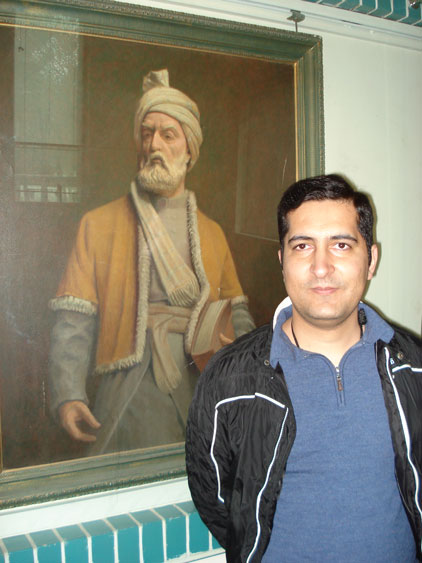
\includegraphics[scale=.5]{Dr_Khaliqi}

\end{figure}

\begin{diagram}[h]
\centering

\includegraphics[scale=.2]{logo}
\caption{دیاگرام تنتبنبلت}
\end{diagram}

\begin{figure}[!ht]
  \centering
  \subfloat[ابوالوفا بوزجانی(ریاضی‌دان و منجم ایرانی)]{\label{sf1}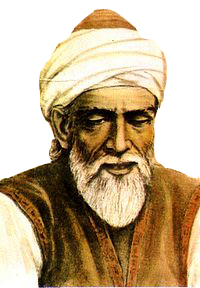
\includegraphics[scale=1.5]{buzjani}}
\quad     \subfloat[دکتر وفا خلیقی(مولف زی‌پرشین)]{\label{sf2}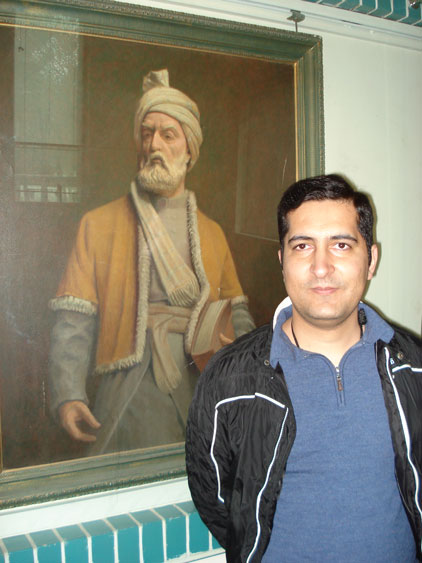
\includegraphics[scale=.26]{Dr_Khaliqi}}\\
    \subfloat[لیزلی لمپارت(مولف لاتک)]{\label{sf3}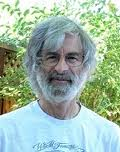
\includegraphics[scale=.9]{LeslieLamport}}
\quad      \subfloat[دونالد کنوث(مولف تک)]{\label{sf4}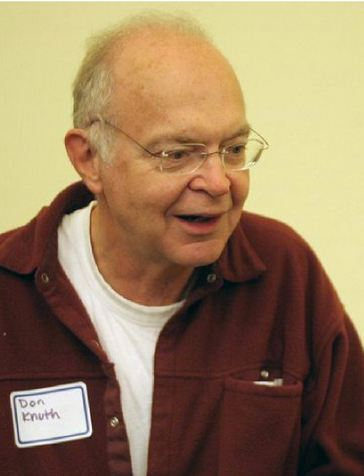
\includegraphics[scale=.29]{knuth}}
  \caption{گذاشتن نمودارها در کنار هم}\label{fi44}
\end{figure}

\ref{sf1}

\clearpage
\subsection{جدول}
به اولین خط جدول توجه ویژه کنید، h و ! دو پارامترهستند که باعث ثابت شدن محیط‌های شناور می‌شوند.

\begin{table}[!ht]
\centering
\caption{می‌توانید در مورد محل عنوان جدول تصمیم‌گیری کنید؟}
\begin{tabular}{lcr}
ردیف &  نام &  نام خانوادگی\\
\hline
$1$ & $2$ & $3$\\
\end{tabular}
\caption{ظاهرامی‌شود.}
\end{table}